% Created 2026-03-04 Wed 19:27
% Intended LaTeX compiler: pdflatex
\documentclass[11pt]{article}

\usepackage[utf8]{inputenc}
\usepackage[T1]{fontenc}
\usepackage{graphicx}
\usepackage{longtable}
\usepackage{wrapfig}
\usepackage{rotating}
\usepackage[normalem]{ulem}
\usepackage{amsmath}
\usepackage{amssymb}
\usepackage{capt-of}
\usepackage{hyperref}
\author{sergio}
\date{\today}
\title{Info Clase}
\hypersetup{
 pdfauthor={sergio},
 pdftitle={Info Clase},
 pdfkeywords={},
 pdfsubject={},
 pdfcreator={},
 pdflang={English}}
\begin{document}

\maketitle
\tableofcontents

\section{Del taller 1 y aclaraciones para el taller 2:}
\label{sec:org65a09dd}

\begin{itemize}
\item El \(\mu = \sqrt{\mu_\alpha^2+\mu_\delta^2}\) es una aproximación
\end{itemize}
Realmente, la corrección es:


\(\mu = \sqrt{(\mu_\alpha cos(\delta))^2 + \mu_\delta^2}\)

\begin{itemize}
\item Gaia da el ángulo en mas, no se cumple:

\(d[pc] = \frac{1}{\pi ('')}\)

Con mas se multiplica por 1000:
\(d[pc] = \frac{1000}{\pi ('')}\)

\item El brillo se atenúa puesto que los instrumentos están en la tierra -> se busca establecer una referencia.
\end{itemize}
\section{La materia prima de los astrónomos es la luz.}
\label{sec:org175e334}

Ondas radio: \(10^3\)

1 Angstrom= 0.10 nm 
\subsection{Magnitud:}
\label{sec:orgfb4844d}

1: Brillante
3.5: Menos brillante
\subsection{Estandarización:}
\label{sec:org9db7bcd}
Placa con orificios.
Mido qué tanto veo por cada hueco pero también mido la distancia.
Los ángulos van cambiando -> brillo depende de la distancia a la que estoy.

\(F \propto \frac{1}{d^2}\)

1 estrella de magnitud 1 es 100 veces más grande que una estrella de magnitud 6.

De 6 a 5: Diferencia de k
De 6 a 4: Diferencia de \(k^2\)
De 6 a 1: \(k^5\)

Así, factor de brillo constante:

\(k^5=100 \longrightarrow k= 2.512 = 10^{2/5}\)

Así, dos estrellas que tengan una diferencia \(\Delta m = m_2 - m_1\) en su magnitud aparente, diferirá su brillo por un factor de:


\(k^{(m_2-m_1)} = \frac{b_1}{b_2} = \frac{F_1}{F_2}\)

Despejando, entonces:

\(m_2-m_1 = 2.5 \log (\frac{F_1}{F_2})\)

Por convención, \(m_1\) es aparente y \(m_2\) es absoluta.

\(m_1 - m_2 = -2.5\log (\frac{F_1}{F_2})\)

Sirve para saber límite de telescopio.


La magnitud más tenue que pued ver con mi ojo es 6:

\(6-m_{lim} = -2.5 \log \frac{D_{tel}^2}{(8mm)^2}\) 

O bien:

\(m_{lim} \approx 1.48 + 5 \log{D_{tel}}\)
\subsection{Módulo de la distancia:}
\label{sec:orga33a45a}

Tenemos:

Escenario A: d\textsubscript{real} y m -> Magnitud aparente
Escenario B: d= 10pc y M -> Magnitud absoluta


\(m-M = -2.5 \log (\frac{F_m}{F_M}) = -2.5 \log (\frac{F_d}{F_{10}}) = -2.5 \log {(\frac{10}{d})}^2\)
Usando leyes de logaritmos, llegamos al \textbf{módulo de la distancia}:
\(m-M = -5 + 5log \, d\)
\section{Taller 3: Topcat - Detección y análisis de cúmilos estelares jóvenes usando GAIA-DR3 (actual)}
\label{sec:orgad36b7d}

Vamos a ir a un cúmulo, ver cuáles están en secuencia principal y cuáles aún son jóvenes.

Se sabe de 2 millones de objetos: Posición, velocidad, brillo, temperatura, composición y tipo. Está en un punto de Lagrange.
\subsection{Filtro fotométrico:}
\label{sec:orgc93c82a}
Filtros pasa bandas MUY anchos.
\section{Apuntes 03-04-2026: Cúmulos estelares.}
\label{sec:org8605b4e}
Satisfacen diferentes cosas:
\begin{itemize}
\item Cinemática compartida
\item Co-espacialidad: Comparten coordenadas similares.
\item Isocronía: Comparten edades parecidas
\item Comparten una huella química.
\item Distribución de masa: Función inicial de masa (IFM) predecible.
\end{itemize}
\subsection{Fundamentos físicos:}
\label{sec:org60de173}
\begin{itemize}
\item Continuidad de Masa.
\item Equilibrio Hidrostático.
\item Transferencia radiativa
\item Balance de Energía: Necesito suficiente masa y temperatura (calor generado por contracción)
\end{itemize}
\subsection{El motor estelar:}
\label{sec:orgd766387}
Debemos tener nucleosíntesis.
La liberación de energía por unidad de masa (q):

\(q=q_0 \rho^m T^m\)

Cuando tengo mayor masa, puedo superar los umbrales de temperatura.

En estrellas como el sol, domina \textbf{combustión de Hidrógeno: Cadenas p-p}.


\begin{center}
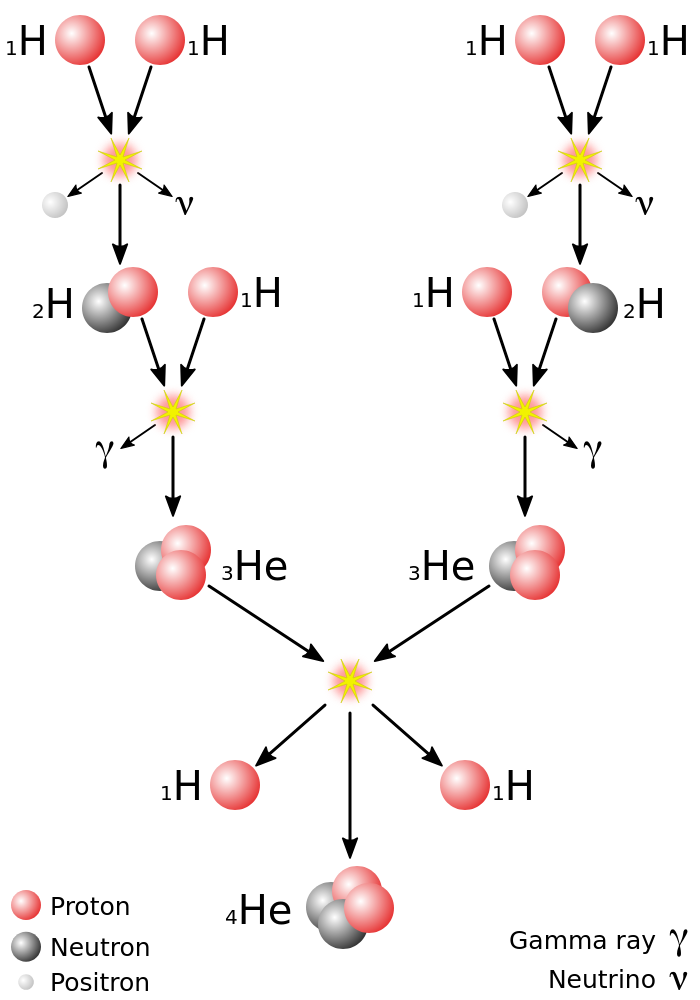
\includegraphics[width=.9\linewidth]{Apuntes_03-04-2026:_Cúmulos_estelares./20260304-183146_screenshot.png}
\end{center}
\textbf{83.3\%} de Helio producido es por ese mecanismo.

Los otros, son generación de Helio-3 con otros elementos ó Helio-4 con Helio-3. Se puede formar Berilio y si no encuentra con quién reaccionar, puede decaer en Litio.

\textbf{Evolución química: Fase Avanzada:} Estrella como capas de cebolla.
\section{Taller:}
\label{sec:orgea50d64}

Vamos a identificar un cúmulo: Queremos identificar cuáles son estrellas jóvenes y cuáles son las adultas, que ya se encuentran sobre la secuencia principal.


Un criterio para clasificar es la edad.

Más masivas, son las que más alumbran y tienen más temperaturas (Parte izquierda del diagrama)
\end{document}
